\ProvidesFile{elliptic_curve.tex}

\section{Эллиптические кривые}
Задаём те же вопросы, бла бла бла.... Короче, нам снова нужны классы эллиптической кривой, точки эллиптической кривой и умные указатели на общие данные.
\subsection{Точка эллиптической кривой}
В реализованном классе используются некие разные виды координат эллиптической кривой и всё такое, но по замерам тестов, они не дают никакого улучшения по времени, а только замедляют, поэтому здесь будет описан только класс эллиптической кривой с нормальными координатами.

\subsubsection{Каркас}
Точка должна содержать свои координаты, числа a, b из уравнения эллиптической кривой:
\[y^2 = x^3 + ax +b\]
Все эти числа лежат в некотором поле $\F_p$, поэтому добавим и его в поля через shared\_ptr. Она должна знать, является ли она точкой $\mathcal{O}$, поэтому добавим поле is\_null. Также, только у класса эллиптической кривой должен быть доступ к конструктору, а значит каркасом будет:
\begin{cppcode}
class EllipticCurvePoint {
    using Element = FieldElement;

    friend class EllipticCurve;

    std::shared_ptr<const Element> m_a;
    std::shared_ptr<const Element> m_b;
    std::shared_ptr<const Field> m_field;

    Element m_x;
    Element m_y;
    bool m_is_null;
};
\end{cppcode}
\subsubsection{Методы}
Что можно делать с точкой?
\begin{itemize}
  \item Создавать:
  Для создания точки надо передать ей все внутренние поля. Чтобы немного оптимизировать создание, сделаем 4 конструктора в зависимости от r-valueльности координат x и y:
  \begin{cppcode}
EllipticCurvePoint(const Element& x, const Element& y, std::shared_ptr<const Element> a,
                   std::shared_ptr<const Element> b, std::shared_ptr<const Field> F,
                   bool is_null = false) :
    m_x(x), m_y(y), m_a(std::move(a)),
    m_b(std::move(b)), m_(std::move(F)), m_is_null(is_null) {};

    EllipticCurvePoint(Element&& x, const Element& y, std::shared_ptr<const Element> a,
                   std::shared_ptr<const Element> b, std::shared_ptr<const Field> F,
                   bool is_null = false) :
    m_x(std::move(x)), m_y(y), m_a(std::move(a)),
    m_b(std::move(b)), m_(std::move(F)), m_is_null(is_null) {};

    EllipticCurvePoint(const Element& x, Element&& y, std::shared_ptr<const Element> a,
                   std::shared_ptr<const Element> b, std::shared_ptr<const Field> F,
                   bool is_null = false) :
    m_x(x), m_y(std::move(y)), m_a(std::move(a)),
    m_b(std::move(b)), m_(std::move(F)), m_is_null(is_null) {};

    EllipticCurvePoint(Element&& x, Element&& y, std::shared_ptr<const Element> a,
                   std::shared_ptr<const Element> b, std::shared_ptr<const Field> F,
                   bool is_null = false) :
    m_x(std::move(x)), m_y(std::move(y)), m_a(std::move(a)),
    m_b(std::move(b)), m_(std::move(F)), m_is_null(is_null) {};
  \end{cppcode}
  Заметим, что мы муваем умные указатели, чтобы атомики внутри них не производили лишнюю работу. Для точки бесконечности мы не поддерживаем никакой специальный вид координат для ускорения работы. То есть имеем "ленивое" обновление координат.
  \item Складывать:
  Чтобы сложить две различные точки, надо провести через них прямую на плоскости и посмотреть, какую точку на эллиптической кривой она пересекла. Тогда симметричная ей точка, относительно оси $Ox$ и будет результатом сложения. Если прямая не пересекла никакую точку на кривой, то считаем, что сумма равна точке $\infty$. Чтобы сложить точку с собой, надо провести касательную через неё и повторить алгоритм выше. Точка $\infty$ будет нулём в данной группе.

    \begin{center}
    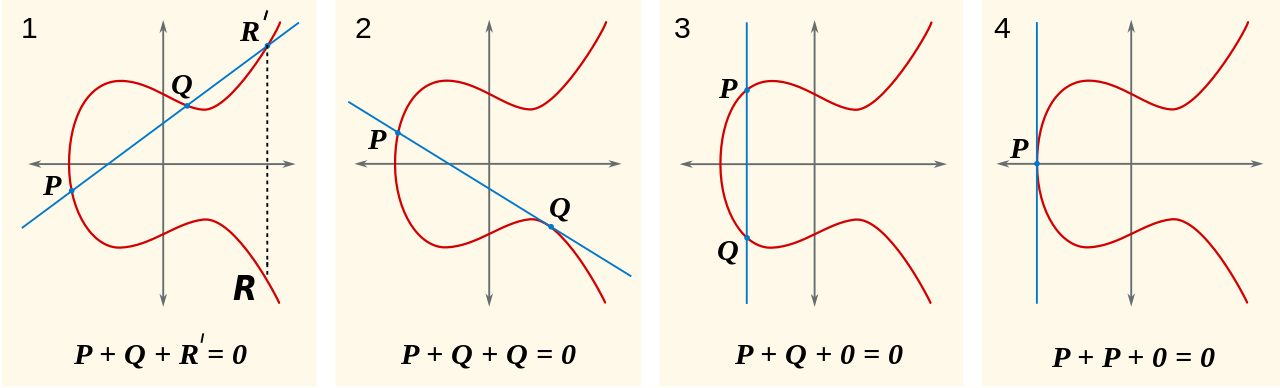
\includegraphics[scale=0.3]{images/ECClines.png} 
    \end{center}

    Заметим, что при таком задании операции '+' обратная точка в группе - это точка с противоположной координатой $y$. С помощью уравнений выразим операцию сложения в нормальных координатах: $A,B,C\in \E(\F_p),\q A=(x_1,y_1),\q B=(x_2,y_2), \q C=(x_3,y_3)$ и $A + B = C$, рассмотрим 3 случая: 
    \begin{enumerate}
      \item $x_1\neq x_2$. Обозначим $k := \frac{y_1-y_2}{x_1-x_2}$. Пусть $C:=A+B$ и $C=(x_3,y_3)$. Тогда
      \[x_3 = k^2 - x_1 - x_2\]
      \[y_3 = k(x_1 - x_3) - y_1\]
      \item $x_1 = x_2,\q y_1 = -y_2$. Тогда $A+B = \infty$.
      \item $A = B$. Обозначим $k := \frac{3x_1^2 + a}{2y_1}$. Тогда
      \[x_3 = k^2 - 2x_1\]
      \[y_3 = k(x_1 - x_3) - y_1\]
    \end{enumerate}

    Определим приватный метод twice для удвоения точки. Заметим, что если $y = 0$, то удвоение точки даст ноль:
    \begin{cppcode}
void twice() {
    if (m_is_null) {
        return;
    }

    if (!m_y.is_invertible()) {
        m_is_null = true;
        return;
    }

    const Element k = (m_field->element(3) * Element::pow(m_x, 2) + *m_a) / (m_y << 1);
    const Element x = Element::pow(k, 2) - (m_x << 1);
    m_y = k * (m_x - x) - m_y;
    m_x = x;
}
    \end{cppcode}
    Значит сложение точки будет:
    \begin{cppcode}
EllipticCurvePoint& operator+=(const EllipticCurvePoint& other) {
    if (m_is_null) {
        return *this = other;
    } else if (other.m_is_null) {
        return *this;
    }

    if (m_x == other.m_x) {
        if (m_y != other.m_y) {
            m_is_null = true;
        } else {
            twice();
        }

        return *this;
    }

    const Element k = (other.m_y - m_y) / (other.m_x - m_x);
    const Element x = Element::pow(k, 2) - m_x - other.m_x;
    m_y = k * (m_x - x) - m_y;
    m_x = x;

    return *this;
}
    \end{cppcode}
    \item Вычитать. Так как мы поняли, что
    \begin{cppcode}
void negative() {
    m_y = -m_y;
}
    \end{cppcode}
    то отрицанием и вычитанием будут:
    \begin{cppcode}
EllipticCurvePoint operator-() const {
    EllipticCurvePoint result = *this;
    result.negative();
    return result;
}

EllipticCurvePoint& operator-=(const EllipticCurvePoint& other) {
    EllipticCurvePoint temp = other;
    temp.negative();
    return *this += temp;
}

EllipticCurvePoint& operator-=(EllipticCurvePoint&& other) {
    other.negative();
    return *this += other;
}
    \end{cppcode}
    \item Умножаться на натуральное число.

    Умножение на число n - это сложение n раз точки с собой. Есть несколько этапов:
    \begin{enumerate}
      \item Представить число n в \textit{non-adjancent form}(NAF) форме - это уникальное представление числа в двоичном основании, где есть цифра $-1$. Такое представление помогает достичть минимального веса Хэмминга (количество цифр, отличных от 0), что заметно ускорит умножение точки на число, если удвоение точки будет быстрее сложения. Алгоритм перевода из двоичной системы исчисления в NAF: 

       \begin{algorithm}[H]
        \caption{NAF from binary}
        \KwData{$n=(n_{m-1}n_{m-2}\dots n_0)_2$}
        \KwResult{$z = (z_{m}z_{m-1}\dots z_1z_0)_{NAF}$}
        $i\gets 0$

        \While{$n > 0$} {
          \eIf{$n$ \rm is odd } {
            $z_i\gets 2 - (n\mod 4)$
            $n\gets n - z_i$
          } {
            $z_i\gets 0$
          }
          $n\gets n/2$

          $i\gets i+1$
        }
      \end{algorithm}
       Есть версия данного алгоритма, которая основана на битовых операциях:

      \begin{algorithm}[H]
        \caption{NAF from binary by bit operations}
        \KwData{$x=(x_{m-1}x_{m-2}\dots n_0)_2$}
        \KwResult{$z = (z_{m}z_{m-1}\dots z_1z_0)_{NAF}$}
        $xh\gets x >> 1$

        $x3\gets x + xh$

        $c\gets xh \text{ XOR } x3$

        $pb\gets x3 \text{ AND } c$

        $nb\gets xh \text{ AND } c$

        $z\gets pb - nb$
      \end{algorithm}
      Есть улучшенная версия данного представления:

      \begin{definition}
        Пусть $w\geqslant 2$ - положительное целое число. Тогда wNAF представление положительного числа $k$ - это представление $k=\sum_{i=0}^{l-1}k_i2^i$, где каждый ненулевой коэффициент $k_i$ нечётный, $|k_i|<2^{w-1}$, $k_{l-1}\neq 0$ и хотя бы одна ненулевая цифра есть в каждой подпоследовательности из $w$ цифр. Длина такого представления равна $l$. 
      \end{definition}
      \begin{theorem}[Свойства wNAF] Пусть $k$ - положительное целое число, тогда 
        \begin{enumerate}
          \item $k$ имеет уникальное представление wNAF, которое обозначается $NAF_w(k)$
          \item $NAF_2(k)=NAF(k)$, где $NAF(k)$ - это классическое бинарное представление в NAF 
          \item Длина $NAF_w(k)$ больше длины $(k)_2$ хотя бы на 1 цифру. 
          \item Средняя плотность ненулевых цифр в $wNAF$ представлении длины $l$ примерно $\frac{1}{w+1}$. 
        \end{enumerate}
      \end{theorem}
      Алгоритм вычисления $wNAF$ формы:

        \begin{algorithm}[H]
        \caption{Computing wNAF}
        \KwData{$w,k\in\N$}
          \KwResult{$NAF_w(k)$}
       $i\gets 0$

          \While{$k\geqslant 1$} {
            \eIf{$k$ is odd } {
              $k_i\gets k$ (mod $2^w$)
              $k\gets k - k_i$
            } {
              $k_i\gets 0$
            }
            $k_i\gets k/2$

            $i\gets i+1$
          }
          \Return $(k_{i-1},\dots,k_1,k_0)$
      \end{algorithm}
      \item Теперь напишем алгоритм вычисления кратной точки:

        \begin{algorithm}[H]
        \caption{wNAF for computing kP}
        \KwData{$w,k\in\N,P\in\E(\F_p)$}
          \KwResult{$Q:=kP$}
          $[k_i]\gets NAF_w(k)$

          Compute $P_i:=iP$ for $i\in \left\{1,3,5,\dots,2^{w-1}-1\right\}$

          $Q\gets \mathcal{O}$

          \For{$i$ from $l-1$ to 0} {
            $Q\gets 2Q$

            \If{$k_i\neq 0$} {
              \eIf{$k_i>0$} {
                $Q\gets Q + P_{k_i}$
              } {
                $Q\gets Q - P_{-{k_i}}$
              }
            }
          }
          \Return $Q$
      \end{algorithm}
    \end{enumerate}
    Имплементируем NAF как шаблон и подружим его с классом точки для быстрого зануления и удвоения:
    \begin{cppcode}
constexpr size_t c_width = 3;

struct Coefficient {
    uint16_t value;
    bool is_negative;
};

using WnafForm = std::vector<Coefficient>;

constexpr uint16_t c_mask_modulo_2_pow_w = (1 << c_width) - 1;

WnafForm get_wnaf(uint value) {
    WnafForm result;

    while (value > 0) {
        if ((value & 0b1) == 1) {
            uint16_t coef_value = value.convert_to<uint16_t>() & c_mask_modulo_2_pow_w;

            if (coef_value >= (1 << (c_width - 1))) {
                coef_value = (1 << c_width) - coef_value;
                result.push_back({.value = coef_value, .is_negative = true});
                value += coef_value;
            } else {
                result.push_back({.value = coef_value, .is_negative = false});
                value -= coef_value;
            }
        } else {
            result.push_back({.value = 0, .is_negative = false});
        }

        value >>= 1;
    }

    return result;
}

constexpr size_t c_k_number = static_cast<size_t>(1) << (c_width - 2);

template<typename T>
T wnaf_addition(T value, const uint& n) {
    WnafForm wnaf_form = get_wnaf(n);
    T two_value = value + value;
    std::vector<T> k_values = {value};

    for (size_t i = 1; i < c_k_number; ++i) {
        k_values.emplace_back(k_values.back() + two_value);
    }

    value.nullify();

    for (size_t i = wnaf_form.size(); i > 0; --i) {
        value.twice();

        if (wnaf_form[i - 1].value != 0) {
            if (!wnaf_form[i - 1].is_negative) {
                value += k_values[wnaf_form[i - 1].value >> 1];
            } else {
                value -= k_values[wnaf_form[i - 1].value >> 1];
            }
        }
    }

    return value;
}
    \end{cppcode}
    где
    \begin{cppcode}
void nullify() {
    m_is_null = true;
}
    \end{cppcode}
    Тогда умножение точки на число будет:
    \begin{cppcode}
EllipticCurvePoint& operator*=(const uint& value) {
    *this = wnaf_addition<EllipticCurvePoint>(*this, value);
    return *this;
}

EllipticCurvePoint& operator*=(const Element& element) {
    *this = wnaf_addition<EllipticCurvePoint>(*this, element.value());
    return *this;
}
    \end{cppcode}
    \item Сравнивать. Точки равны, если они обе нули или если у них совпадают координаты:
    \begin{cppcode}
friend bool operator==(const EllipticCurvePoint& lhs, const EllipticCurvePoint& rhs) {
    return (lhs.m_is_null && rhs.m_is_null) || (lhs.m_x == rhs.m_x && lhs.m_y == rhs.m_y);
}
    \end{cppcode}
    \item Приватный статический метод создания нулевой точки. За нулевую точку принято считать точку с координатами (0,1):
    \begin{cppcode}
static EllipticCurvePoint null_point(const std::shared_ptr<const Element>& a,
const std::shared_ptr<const Element>& b, const std::shared_ptr<const Field>& F) {
          return EllipticCurvePoint(F->element(0), F->element(1), a, b, F, true);
}    
    \end{cppcode}
    \item Стандартным образом определяем по 4 дружественных оператора на каждую операцию $+,-,*$ через их $+=$ версии.
    \item Делаем геттеры на x,y.
\end{itemize}
\subsection{Эллиптическая кривая}
По сути мы повторяем функционал класса поля:
\begin{cppcode}
class EllipticCurve {
    using Field = field::Field;
    using Element = field::FieldElement;

public:
    EllipticCurve(const Element& a, const Element& b, Field F);
    EllipticCurve(Element&& a, const Element& b, Field F);
    EllipticCurve(const Element& a, Element&& b, Field F);
    EllipticCurve(Element&& a, Element&& b, Field F);

    const Field& get_field() const;
    const Element& get_a() const;
    const Element& get_b() const;

private:
    std::shared_ptr<const Element> m_a;
    std::shared_ptr<const Element> m_b;
    std::shared_ptr<const Field> m_field;
};
\end{cppcode}
Этот класс должен поддерживать 3 вида создания точек:
\begin{itemize}
  \item Создание нулевой точки:
  \begin{cppcode}
EllipticCurvePoint null_point() const {
    return EllipticCurvePoint::null_point(m_a, m_b, m_field);
}
  \end{cppcode}
  \item Создание точки от x координаты. Но на эллиптической кривой может и не лежать данная координата, поэтому надо проверить, существует ли корень от $x^3 + ax + b$ в $\F_p$. Есть два варианта:
  \begin{enumerate}
    \item $p\equiv 3\mod 4$
    \item $p\equiv 1\mod 4$
  \end{enumerate}
  Почти все простые числа от NIST обладают первым свойством, поэтому рассмотрим только его. Но в реализации имплементирован и протестирован и второй случай.
  \begin{enumerate}
    \item Если число $a$ имеет корень $x\in\F_p\colon x^2 = a$, то $a$ либо равен 0, тогда корень понятно 0, либо лежит в $2\Z_{p - 1}$, так как $\F_p^*\cong \Z_{p-1}$.

  Пусть $p - 1=: 2k$. Значит $k = \frac{p-1}{2}$. Заметим, что тогда 
  \[\forall y \in 2\Z_{p - 1}\q \frac{p-1}{2}y = 0\] 
  Отсюда вытекает критерий: $\exists x\in\F_p\colon x^2 = a \Leftrightarrow a^{\frac{p-1}{2}} = 1$.
    \item Пусть $a^{\frac{p-1}{2}} = 1$. Так как $p\equiv 3\mod 4$, то $\frac{p-1}{2}$ нечётно, т.е.
    \[\frac{p-1}{2} = 2k - 1\implies \frac{p+1}{2} = 2k\]
    Тогда получаем, что
    \[a^{\frac{p-1}{2}} = 1\implies a^{\frac{p-1}{2}}\cdot a = a\]
    \[a = a^{\frac{p+1}{2}} = a^{2k}=(a^k)^2\]
    Значит в качестве корня подойдёт $x:= a^k = a^{\frac{p+1}{4}}$.

    Итого:
    \begin{cppcode}
std::optional<FieldElement> find_root(const FieldElement& value, const Field& field) {
    if (!value.is_invertible()) {
        return std::nullopt;
    }

    const uint& p = field.modulus();
    const FieldElement one = field.element(1);

    if (FieldElement::pow(value, (p - 1) >> 1) != one) {
        return std::nullopt;
    }

    return FieldElement::pow(value, (p + 1) >> 2);
}
    \end{cppcode}
    Используем std::optional для передачи того, можно ли найти корень или нет. Тогда методами эллиптической кривой будут:
    \begin{cppcode}
private:
std::optional<EllipticCurve::Element> EllipticCurve::find_y(const Element& x) const {
    Element value = Element::pow(x, 3) + *m_a * x + *m_b;
    return find_root(value, *m_field);
}

public:
std::optional<EllipticCurvePoint> point_with_x_equal_to(const Element& x) const {
    if (!x.is_invertible()) {
        return null_point();
    }

    std::optional<Element> y = find_y(x);

    if (!y.has_value()) {
        return std::nullopt;
    }

    return EllipticCurvePoint(x, std::move(y.value()), m_a, m_b, m_field);
}

std::optional<EllipticCurvePoint> point_with_x_equal_to(Element&& x) const {
    if (!x.is_invertible()) {
        return null_point();
    }

    std::optional<Element> y = find_y(x);

    if (!y.has_value()) {
        return std::nullopt;
    }

    return EllipticCurvePoint(std::move(x), std::move(y.value()), m_a, m_b, m_field);
}
    \end{cppcode}
    \item Создание точки по двум координатам. Надо проверить только, что координаты удовлетворяют уравнению кривой:
    \begin{cppcode}
private:
bool EllipticCurve::is_valid_coordinates(const Element& x, const Element& y) const {
    const Element lhs = Element::pow(y, 2);
    const Element rhs = Element::pow(x, 3) + *m_a * x + *m_b;
    return lhs == rhs;
}

bool EllipticCurve::is_null_coordinates(const Element& x, const Element& y) const {
    return x.value() == 0 && y.value() == 1;
}

public:
std::optional<EllipticCurvePoint> point(const Element& x, const Element& y) const {
    if (is_null_coordinates(x, y)) {
        return null_point();
    }

    if (!is_valid_coordinates(x, y)) {
        return std::nullopt;
    }

    return EllipticCurvePoint(x, y, m_a, m_b, m_field);
}

std::optional<EllipticCurvePoint> point(Element&& x, const Element& y) const {
    if (is_null_coordinates(x, y)) {
        return null_point();
    }

    if (!is_valid_coordinates(x, y)) {
        return std::nullopt;
    }

    return EllipticCurvePoint(std::move(x), y, m_a, m_b, m_field);
}

std::optional<EllipticCurvePoint> point(const Element& x, Element&& y) const {
    if (is_null_coordinates(x, y)) {
        return null_point();
    }

    if (!is_valid_coordinates(x, y)) {
        return std::nullopt;
    }

    return EllipticCurvePoint(x, std::move(y), m_a, m_b, m_field);
}

std::optional<EllipticCurvePoint> point(Element&& x, Element&& y) const {
    if (is_null_coordinates(x, y)) {
        return null_point();
    }

    if (!is_valid_coordinates(x, y)) {
        return std::nullopt;
    }

    return EllipticCurvePoint(std::move(x), std::move(y), m_a, m_b, m_field);
}
    \end{cppcode}
  \end{enumerate}
\end{itemize}

